\graphicspath{{$HOME/TFG/Graphics/Cpt1-Charactz/}}

		\begin{figure}[H]
			\centering
			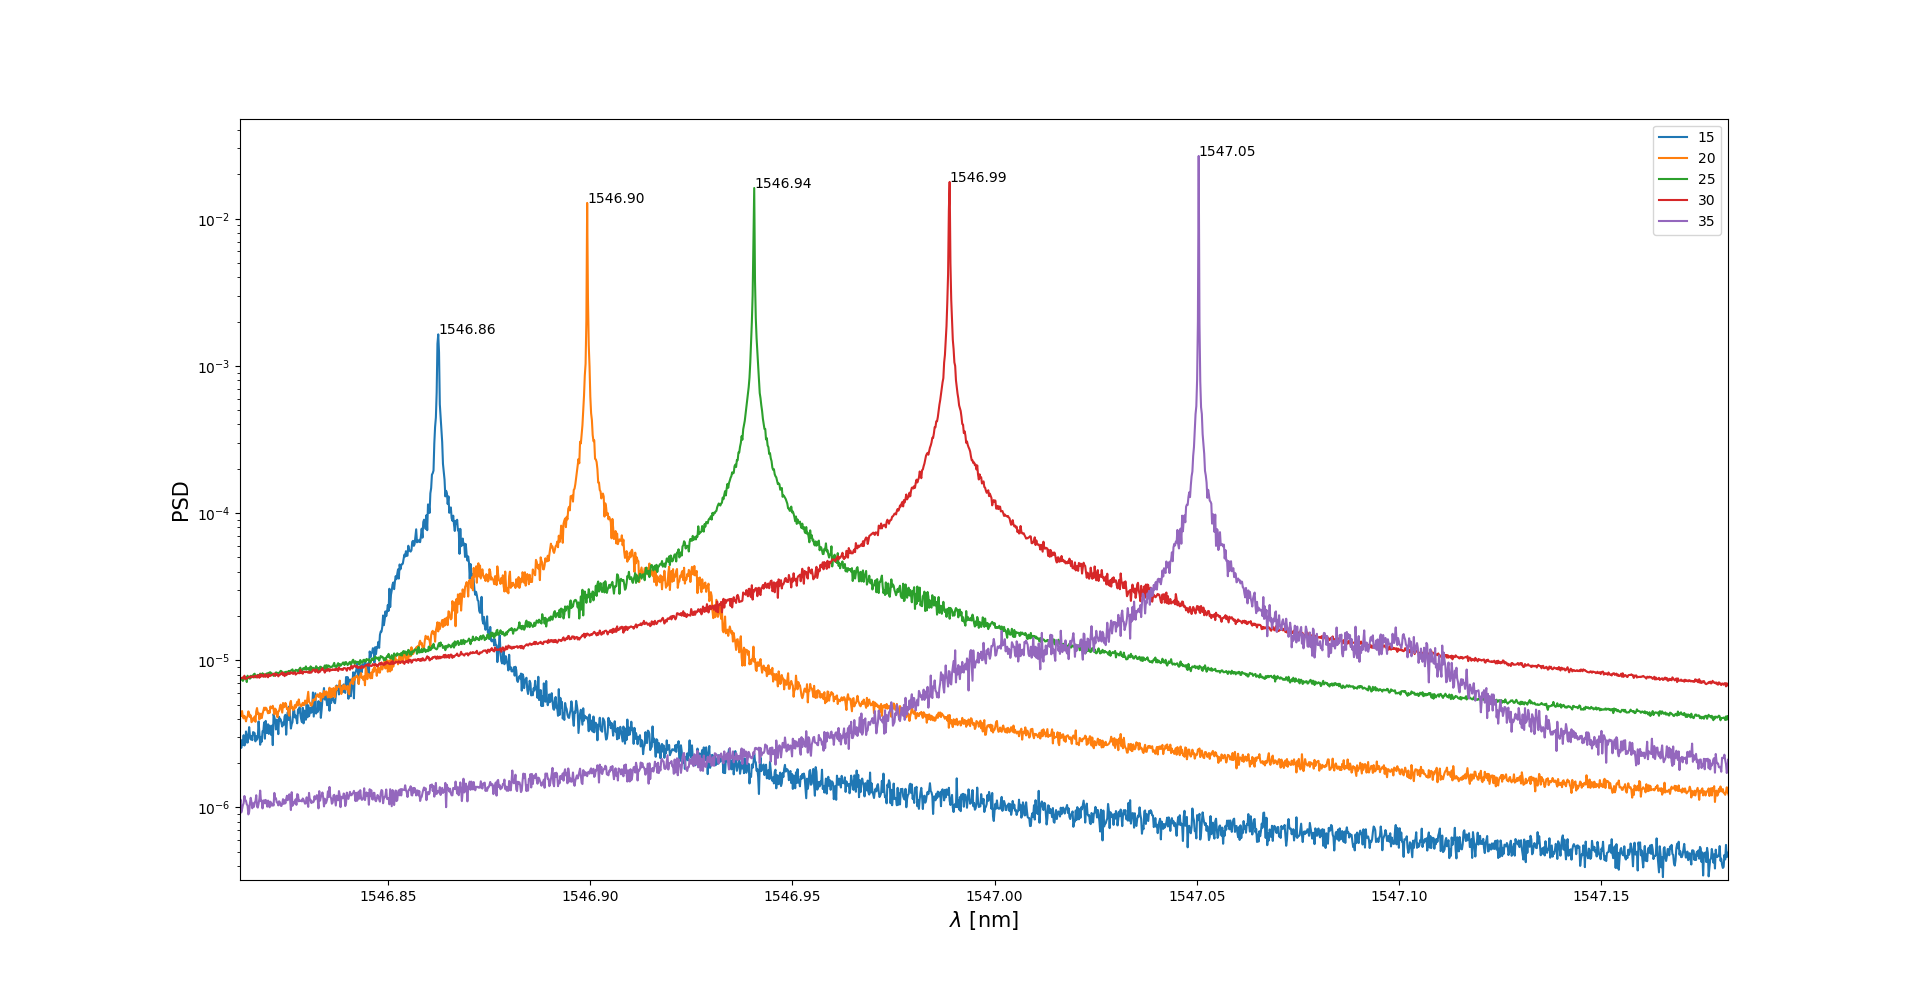
\includegraphics[width=1.0\linewidth]{Espectros.png}
			\caption{\label{Img:widgets}Espectros en continua de la simulacion}
		\end{figure}

		\begin{table}[H]
			\centering
			\begin{tabular}{c c}
				\hline
				$I_{Bias}$ & $\lambda$ \\\hline 
				15 & 1546.86 \\
				20 & 1546.90 \\
				25 & 1546.94 \\
				30 & 1546.99 \\
				35 & 1547.05 \\\hline
			\end{tabular}
			\caption{\label{tab:label}Lambdas de la simulacion}
		\end{table}

		\begin{figure}[H]
			\centering
			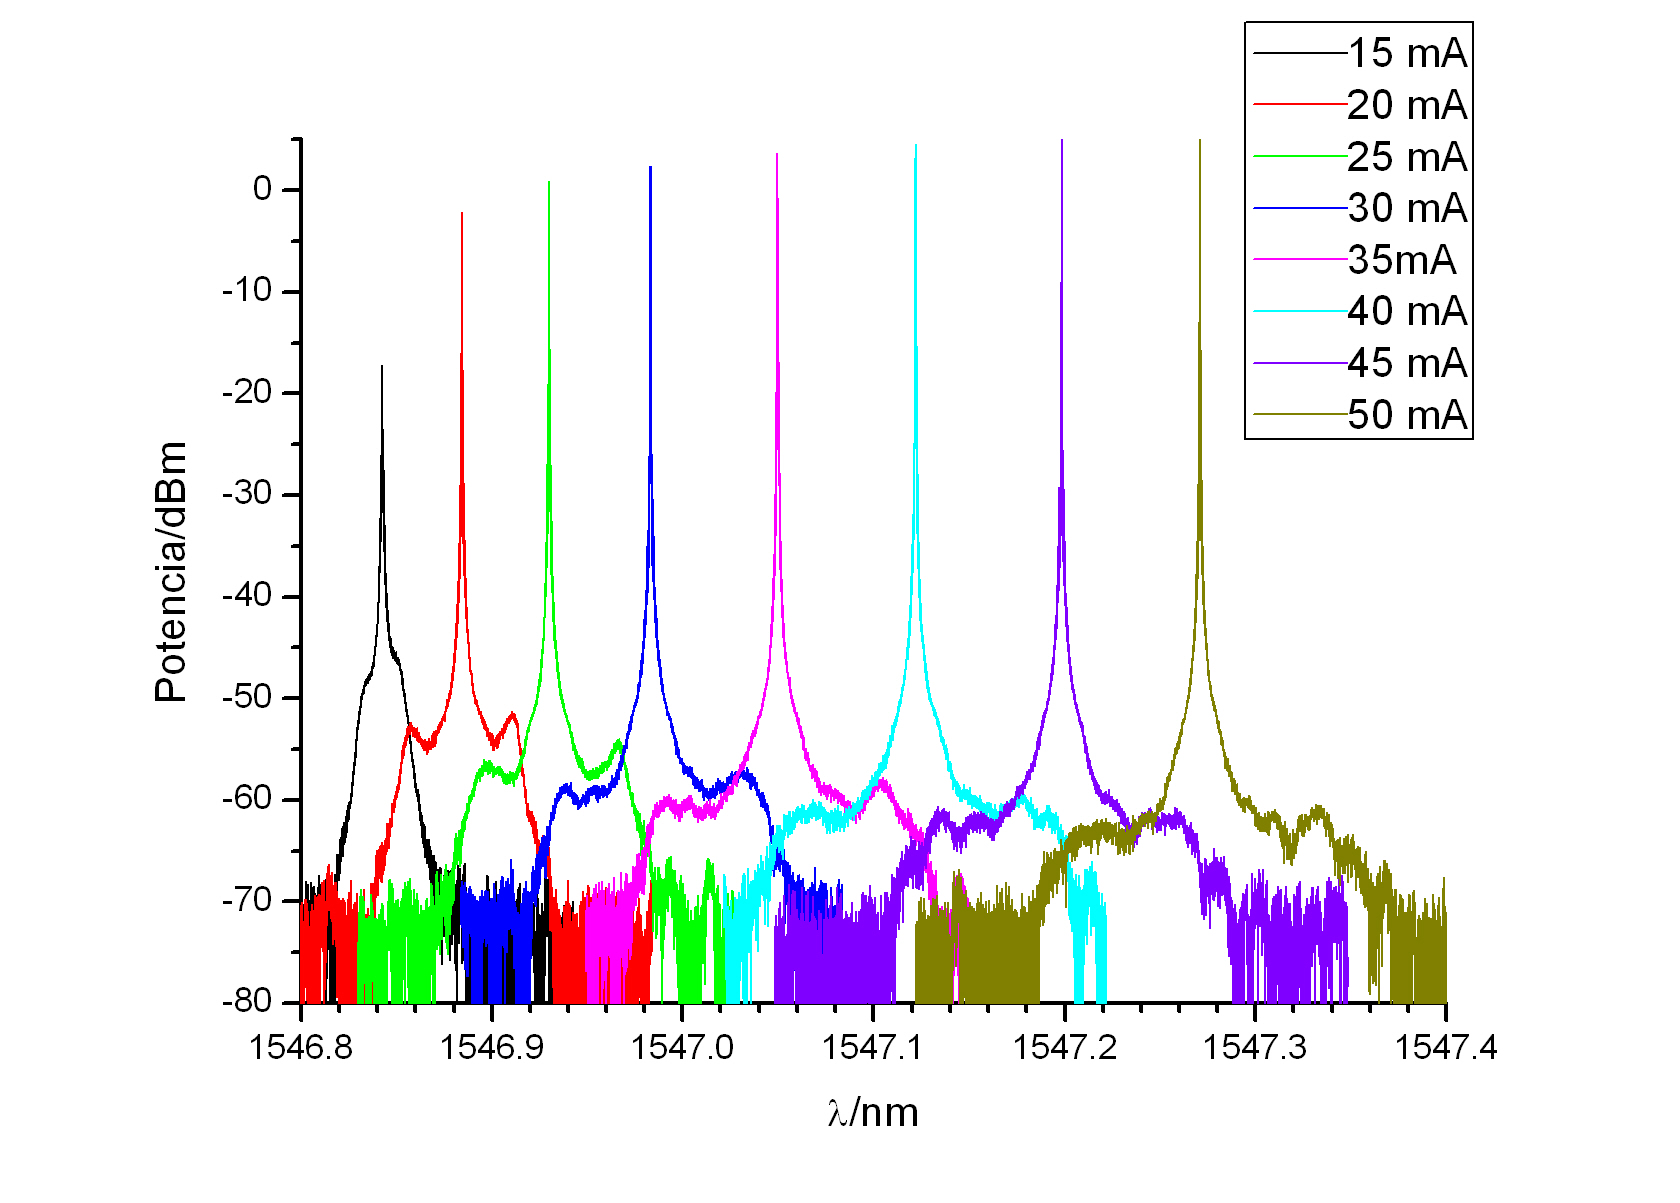
\includegraphics[width=1.0\linewidth]{../Chaves/OFC-GS/EspectrosT25.jpg}
			\caption{\label{fig:EspectrosT25}Espectros en continua de Chaves}	
		\end{figure}
	

		\begin{figure}[H]
			\centering
			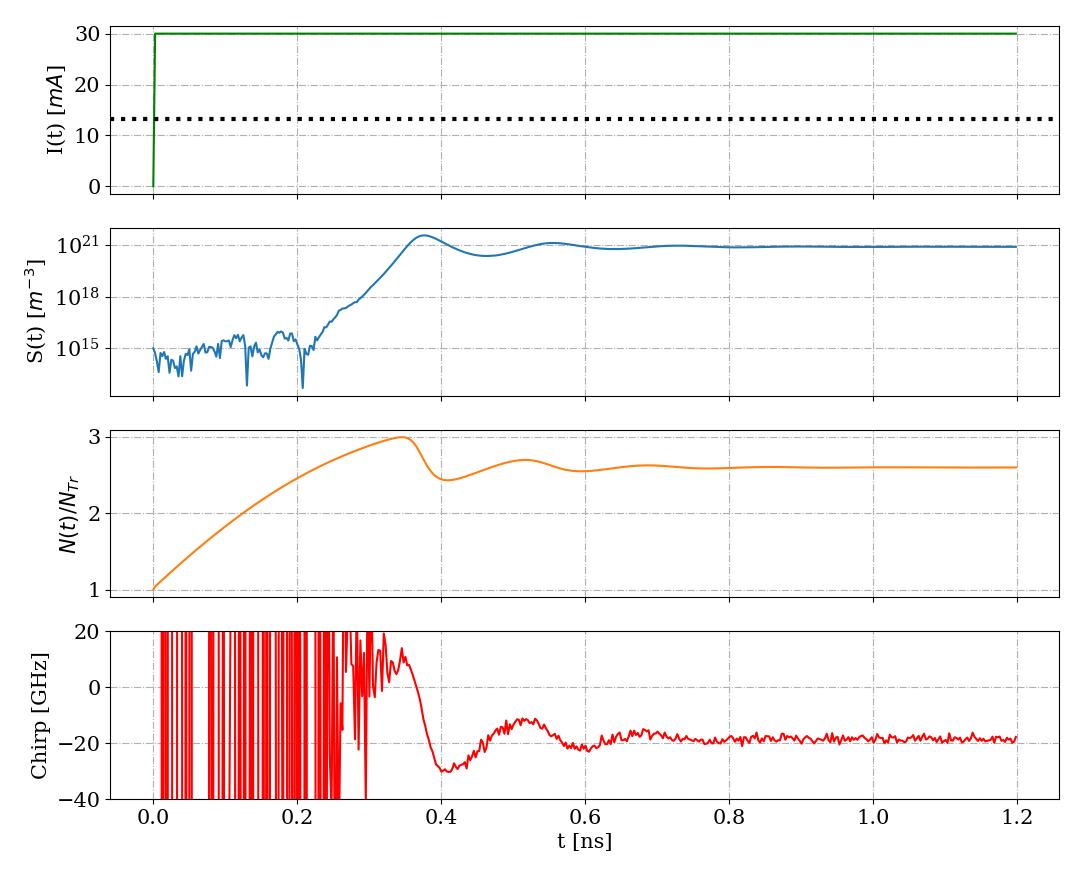
\includegraphics[width=1.0\linewidth]{transitorio.png}
			\caption{\label{fig:transitorio}Transitorio}	
		\end{figure}

		\begin{figure}[H]
			\centering
			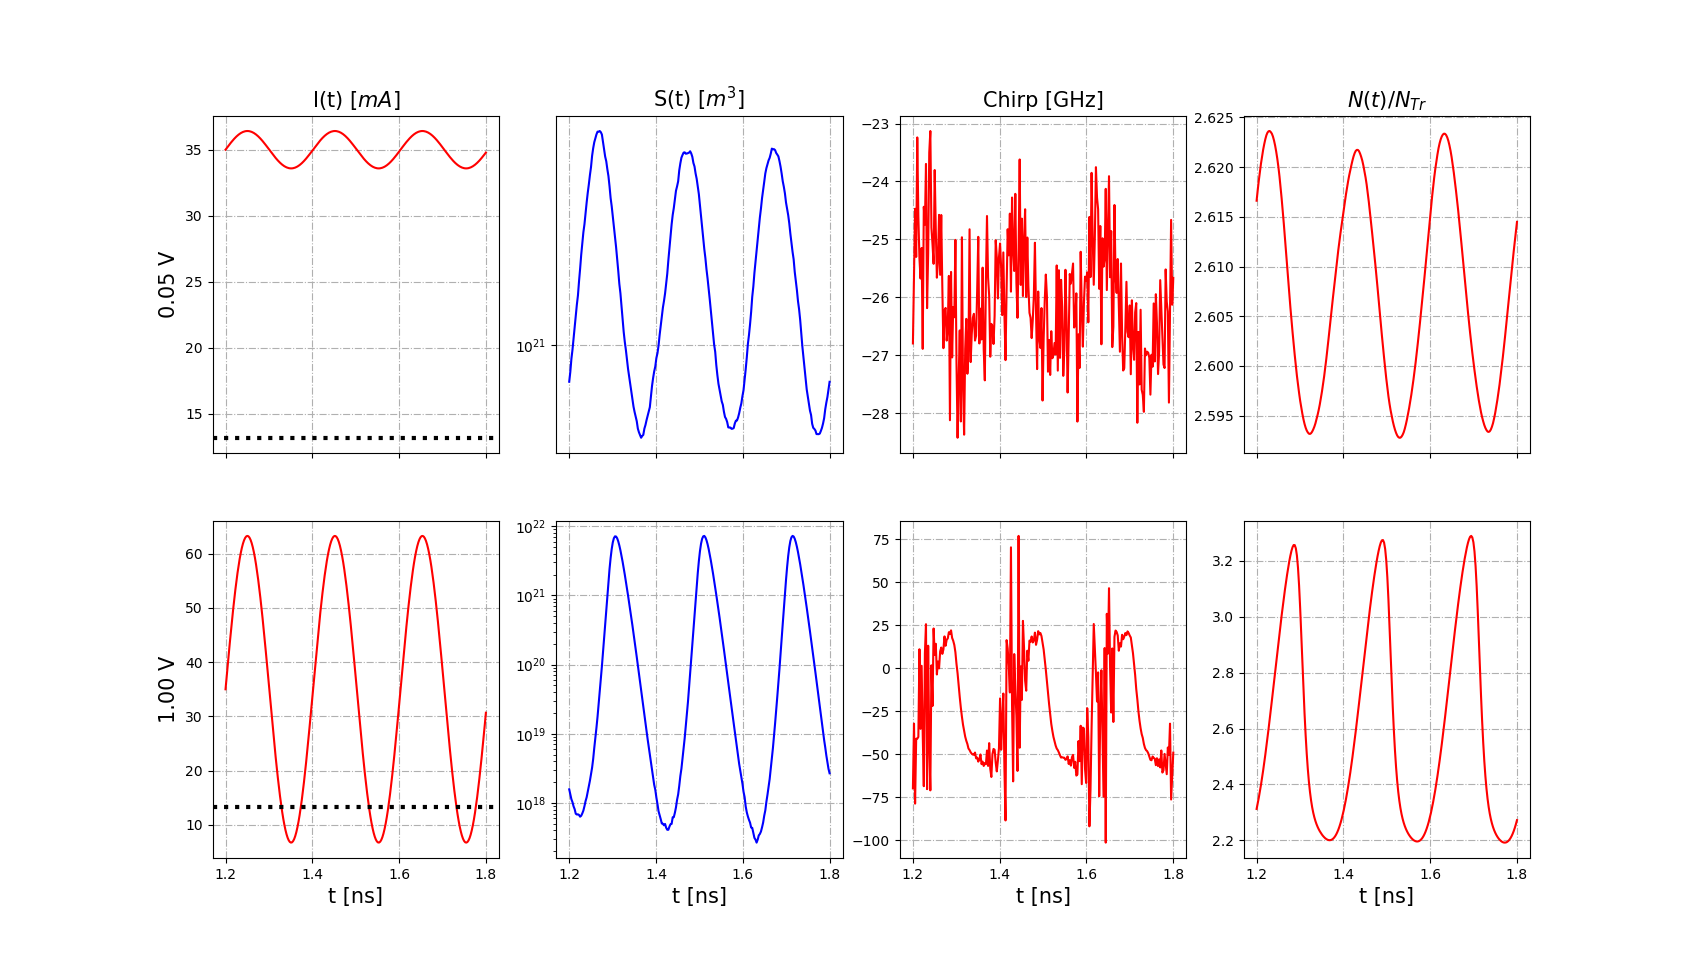
\includegraphics[width=1.0\linewidth]{rateEquations.png}
			\caption{\label{fig:rateEquations}RateEquations}	
		\end{figure}

		\begin{figure}[H]
			\centering
			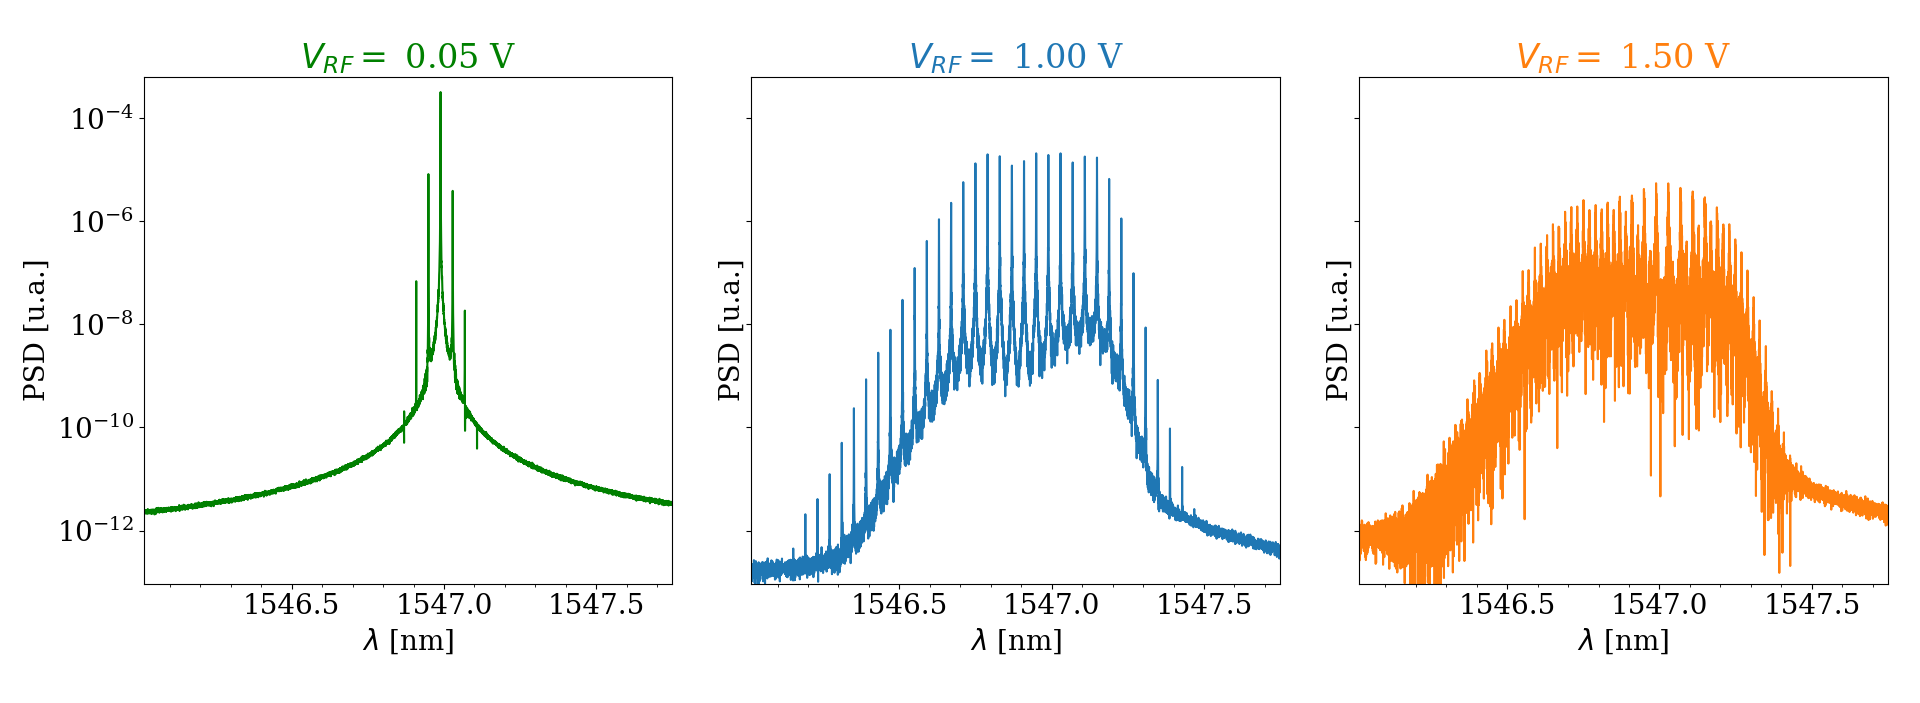
\includegraphics[width=1.0\linewidth]{PSD.png}
			\caption{\label{fig:PSD}PSD}	
		\end{figure}

		\begin{figure}[H]
			\centering
			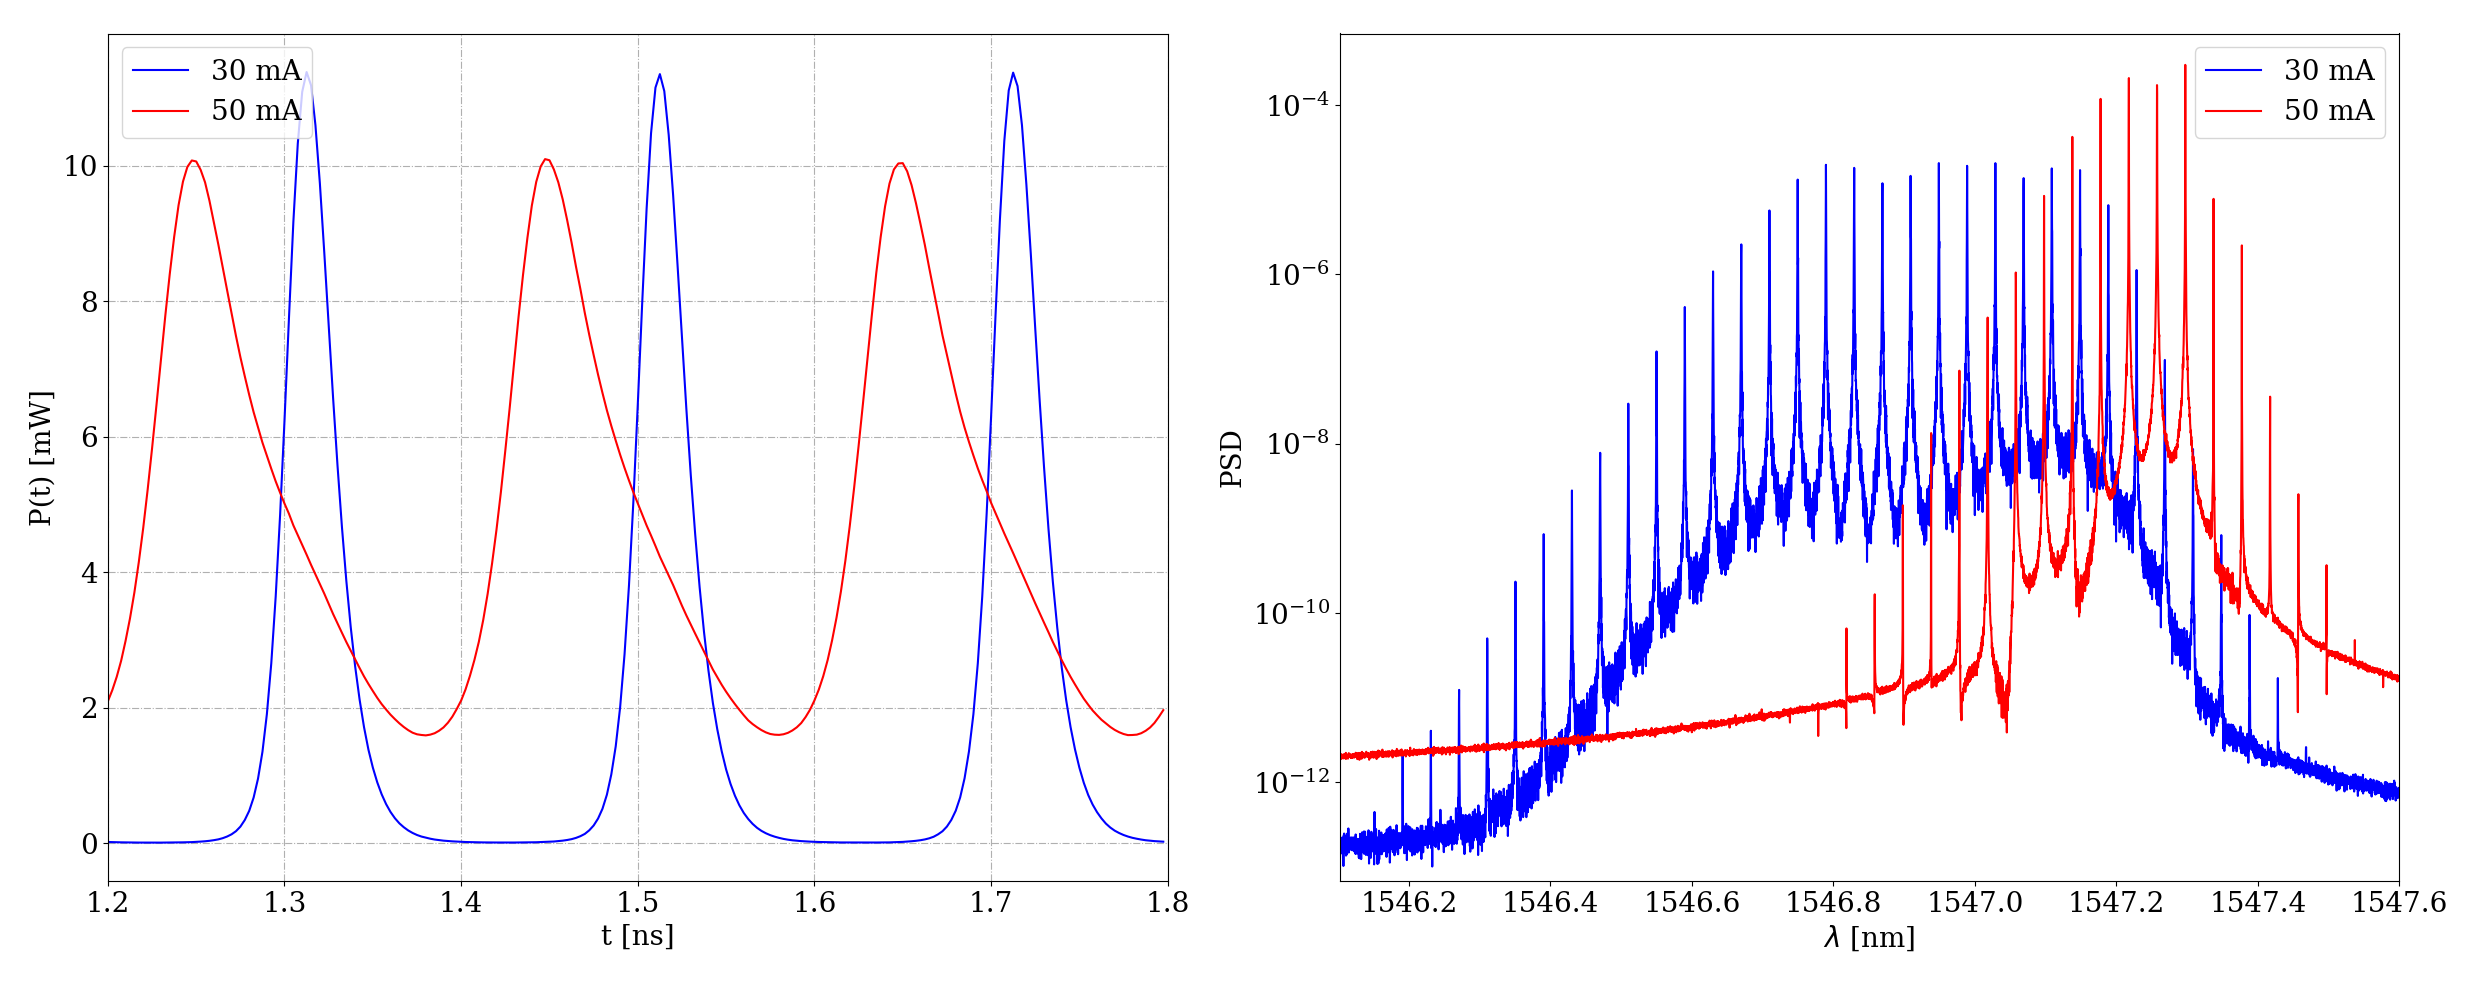
\includegraphics[width=1.0\linewidth]{current.png}
			\caption{\label{fig:current}Current}	
		\end{figure}

		\begin{figure}[H]
			\centering
			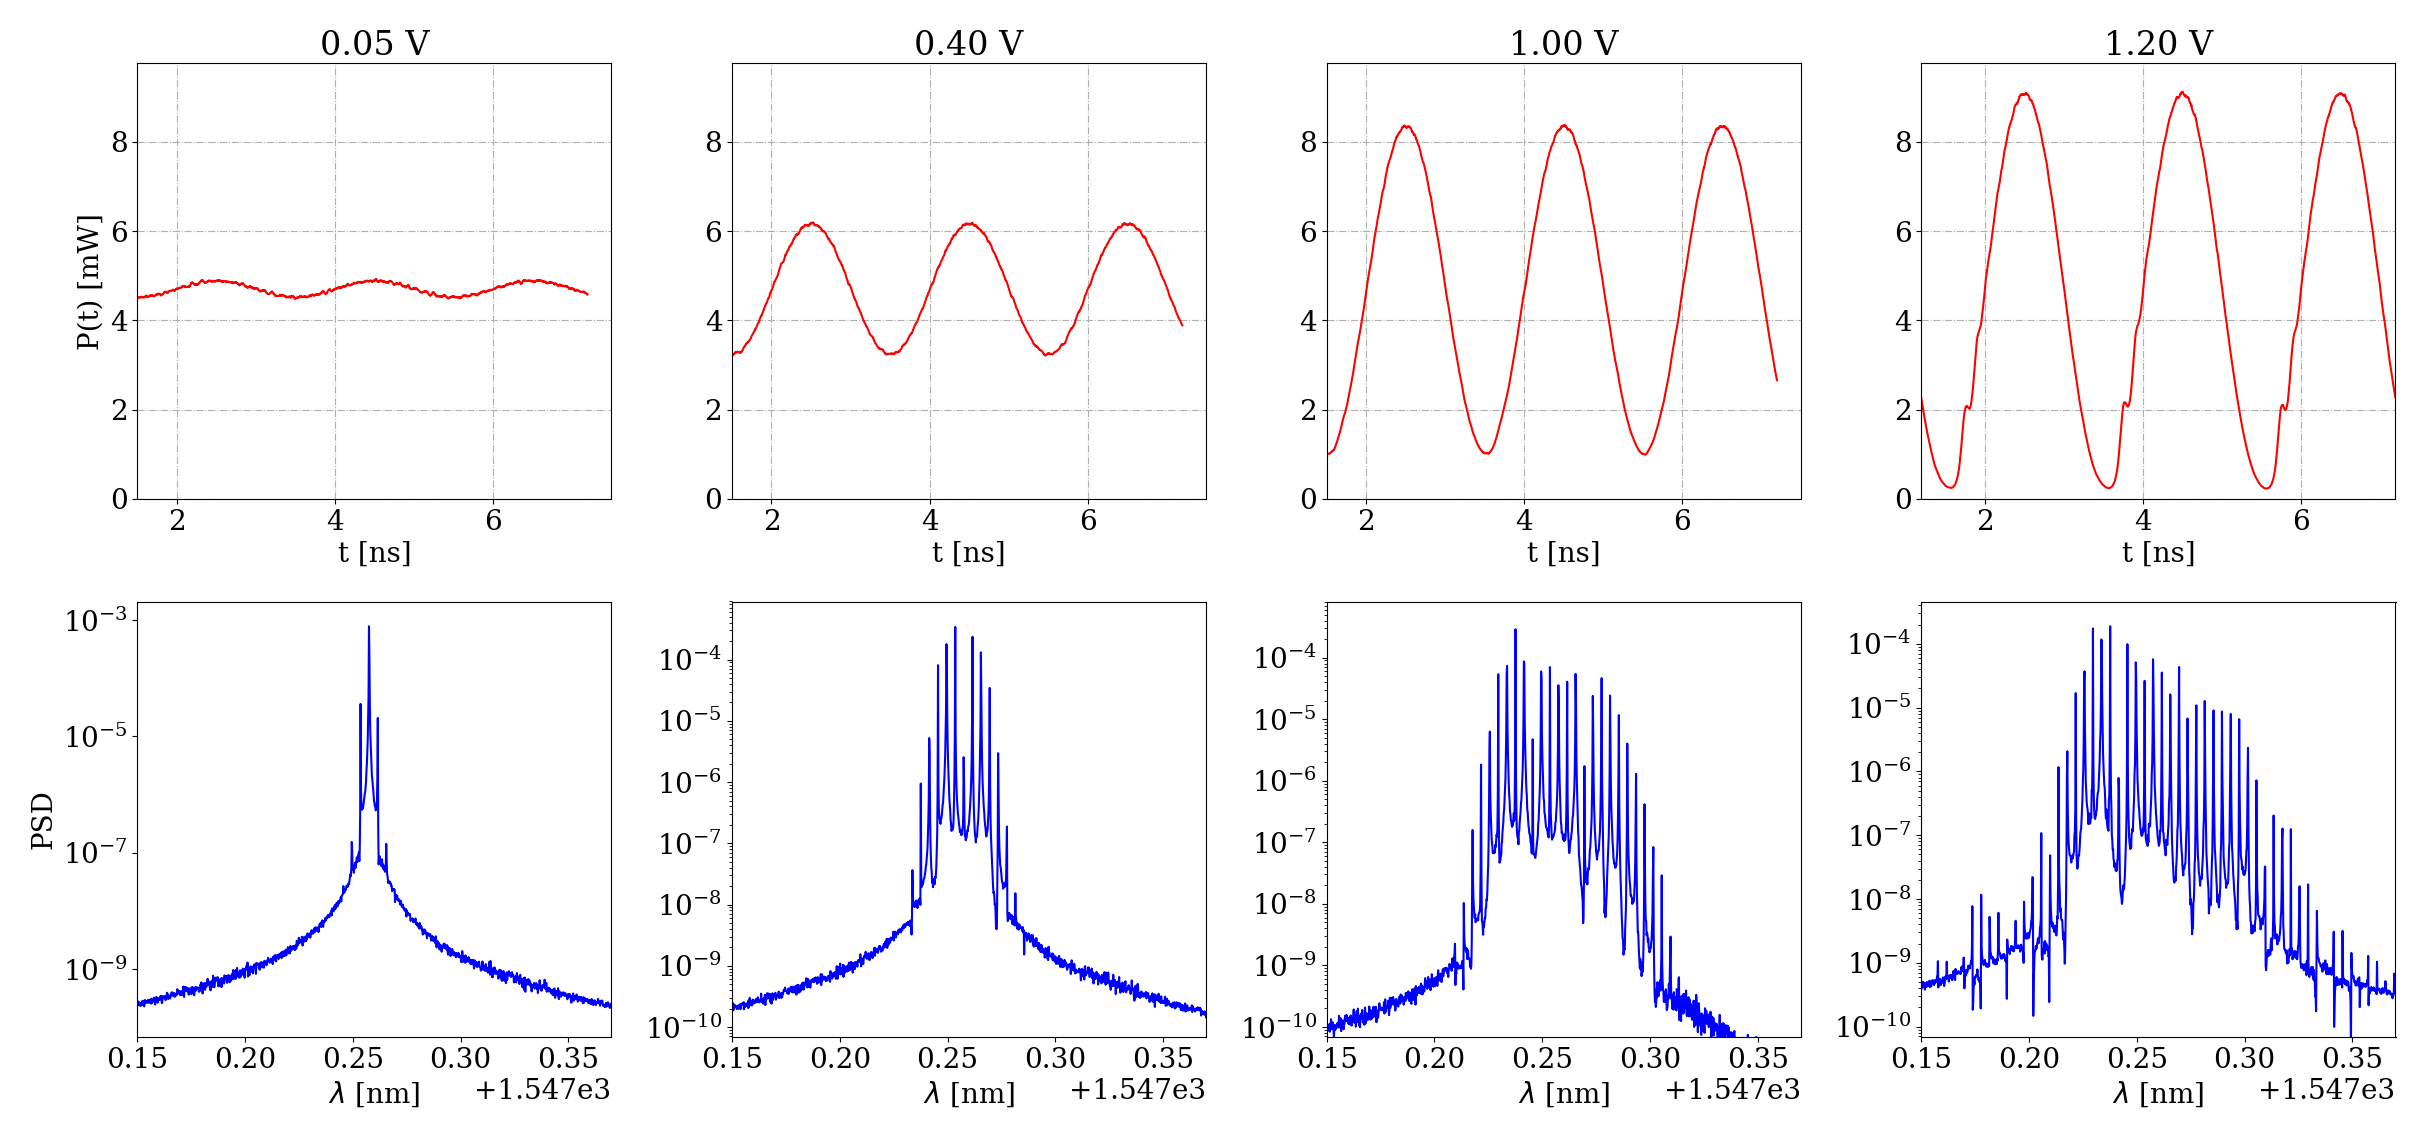
\includegraphics[width=1.0\linewidth]{500.png}
			\caption{\label{fig:500}500}	
		\end{figure}

		\begin{figure}[H]
			\centering
			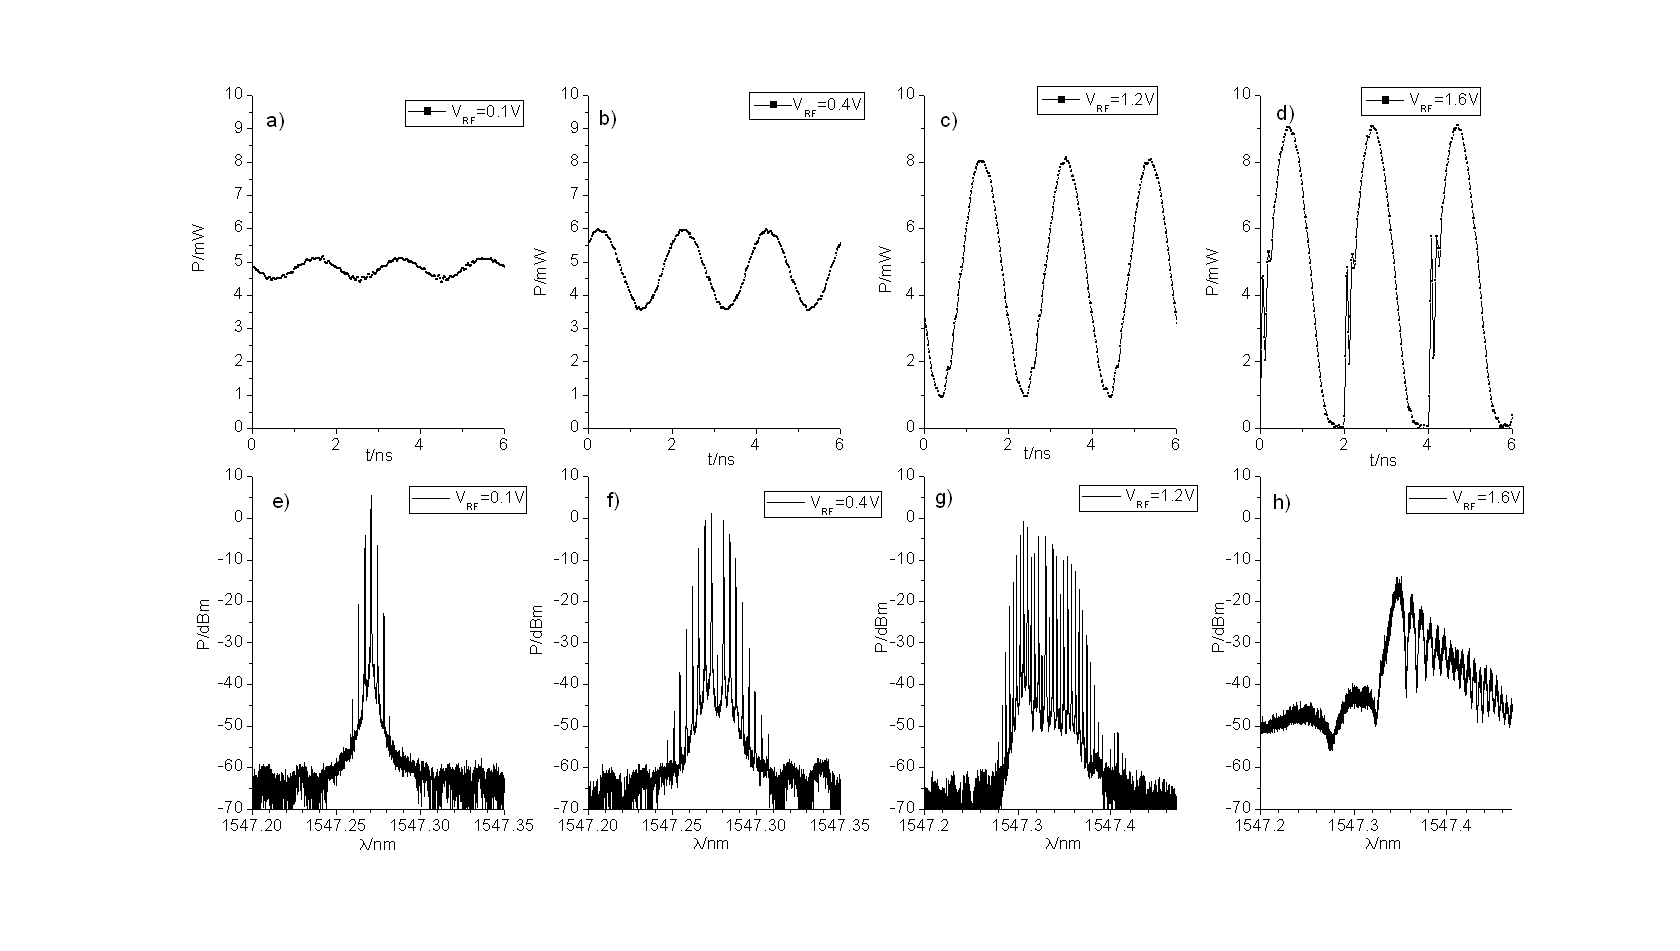
\includegraphics[width=1.0\linewidth]{../Chaves/OFC-GS/500mhz.png}
			\caption{\label{fig:500mhz}500mhz}	
		\end{figure}
